\documentclass[12pt]{article}

\usepackage[utf8]{inputenc}
\usepackage[T1]{fontenc}

\usepackage{amsmath, amssymb}
\usepackage{geometry}
\geometry{margin=1in}

\usepackage{graphicx}
\usepackage{float}
\usepackage[section]{placeins}

\usepackage{caption}
\captionsetup{font=small, labelfont=bf, skip=6pt}
\usepackage{booktabs,tabularx}
\newcolumntype{Y}{>{\raggedright\arraybackslash}X}

\usepackage{hyperref}

\usepackage[backend=biber,style=numeric,sorting=none]{biblatex}
\addbibresource{references.bib}

\usepackage{microtype}

\setlength{\textfloatsep}{10pt plus 2pt minus 2pt}
\setlength{\floatsep}{8pt plus 2pt minus 2pt}
\setlength{\intextsep}{10pt plus 2pt minus 2pt}
\setlength{\abovecaptionskip}{6pt}
\setlength{\belowcaptionskip}{0pt}

\title{A Cyclic 4D-Time Universe Model: Bounce, Expansion, and Turnaround Controlled by Closed Time Geometry}
\author{Jacob L. Powell}
\date{\today}

\begin{document}
\maketitle

\begin{abstract}
We propose a conceptual cosmological framework in which the fourth dimension---time---is
not infinite, but cyclic and bounded. This closed time geometry provides a natural mechanism
for both the initiation of cosmic expansion (the bounce) and its termination (the turnaround),
removing the need for external triggers. We derive an effective Friedmann equation, inspired by
Loop Quantum Cosmology (LQC), that incorporates quantum corrections to avoid singularities,
and show how a large-$a$ turnaround can arise through curvature or an effective negative
cosmological term. The bounce is interpreted as a single-frame quantum state, linking emergent
time concepts with cyclic and conformal cosmological models. We highlight how this approach
differs from both LQC and Conformal Cyclic Cosmology (CCC), and sketch potential observational
signatures in the CMB and primordial gravitational waves. While speculative, the closed-time
ansatz yields falsifiable predictions in principle and motivates further work on entropy bounds
and observational signatures.
\end{abstract}

\section{Introduction}
The classical theory of general relativity predicts singularities at the Big Bang and inside
black holes, where the equations cease to be valid. Loop Quantum Cosmology (LQC) provides
a resolution through quantum corrections that replace singularities with bounces
\cite{Ashtekar2006,Bojowald2001}. Other cyclic approaches, such as the ekpyrotic/cyclic
scenario \cite{Steinhardt2002}, posit a sequence of universes but often leave the termination
of expansion unspecified. Penrose's Conformal Cyclic Cosmology (CCC) \cite{Penrose2010}
offers an alternative by identifying the remote future of one aeon with the Big Bang of the
next through conformal rescaling.

The proposal developed here differs in a key way: time itself is treated as a closed arc,
with expansion and contraction bounded by its periodicity. This \emph{cyclic 4D-time} ansatz
eliminates the need for ad hoc triggers and provides a unified geometric controller for both
the bounce and the turnaround.

\section{Framework}
\subsection{Cyclic Time Ansatz}
We posit periodic cosmic time $\tau\in[0,T)$ such that $a(\tau+T)=a(\tau)$. Turning points
occur at $a_{\min}$ (bounce) and $a_{\max}$ (turnaround), where $\dot a=0$.
It is convenient to define an effective potential
\begin{equation}
\dot a^2 + U(a) = 0, \qquad
U(a) \equiv -\,a^2\!\left[\frac{8\pi G}{3}\rho(a)\left(1-\frac{\rho(a)}{\rho_c}\right)-\frac{k}{a^2}\right].
\end{equation}
The cycle period is
\begin{equation}
T = 2\int_{a_{\min}}^{a_{\max}}\frac{da}{\sqrt{-U(a)}},
\end{equation}
which is finite if both turning points exist.

\subsection{Effective Friedmann Equation from a Hamiltonian}
Following LQC, the effective Hamiltonian constraint is
\begin{equation}
\mathcal{C}_{\rm eff}
= -\frac{3}{8\pi G\,\gamma^2\lambda^2}\, a^3 \sin^2(\lambda b) + \rho(a)\,a^3 = 0,
\end{equation}
with Barbero--Immirzi parameter $\gamma$ and area gap $\lambda=\sqrt{\Delta}$.
This yields
\begin{equation}
H^2=\frac{8\pi G}{3}\rho(a)\left(1-\frac{\rho(a)}{\rho_c}\right)-\frac{k}{a^2}, \qquad
\rho_c=\frac{3}{8\pi G\,\gamma^2\,\lambda^2}.
\end{equation}
\textit{Convention.} We set $\Lambda=0$ to avoid double counting; all vacuum-like terms,
including closed-time effects, are absorbed into $\rho(a)$.

\paragraph{Bounce.}
At $a=a_{\min}$, $H=0$ implies $\rho=\rho_c$. Using the effective Raychaudhuri equation,
\[
\dot H = -4\pi G(\rho+P)\!\left(1-2\frac{\rho}{\rho_c}\right)+\frac{k}{a^2},
\]
one finds $\dot H>0$ for $k=0$ and $\rho+P>0$, confirming stability.

\paragraph{Turnaround.}
At $a=a_{\max}$, $H=0$ implies
\[
\frac{8\pi G}{3}\rho(a_{\max})\left(1-\frac{\rho(a_{\max})}{\rho_c}\right)-\frac{k}{a_{\max}^2}=0.
\]
A turnaround may therefore be achieved either by (i) a negative effective vacuum term
(as introduced below), (ii) positive curvature $k=+1$, or (iii) a bare negative $\Lambda$.
In this model, we interpret the effective negative term as a consequence of compact time.

\subsection{Closed Time as Effective Dynamics}
Compactifying cosmic time as $\tau\in S^1$ motivates an additional contribution.
We adopt a phenomenological ansatz
\begin{equation}
\rho_{\rm CT}(R_\tau) = -\frac{\sigma}{R_\tau^4}, \qquad R_\tau=T/2\pi.
\end{equation}
This negative scaling ensures a turnaround at large $a$, with effective
$\Lambda_{\rm eff}=8\pi G\,\rho_{\rm CT}<0$.
\emph{Remark.} In QFT, compact Euclidean time yields a positive $\propto T^4$ energy density;
hence the negative sign here is an assumption requiring future derivation.

We also allow a mild $R_\tau$-dependence of the polymer scale,
\[
\rho_c(R_\tau)=\frac{3}{8\pi G\,\gamma^2\,\tilde\lambda^2(R_\tau)},\quad
\tilde\lambda^2(R_\tau)=\lambda^2\Big[1+\chi\Big(\tfrac{\ell_{\rm P}}{R_\tau}\Big)^2+\cdots\Big].
\]

\paragraph{Cycle quantization (heuristic).}
A Bohr--Sommerfeld-type condition,
\[
\oint p_a\,da = 2\pi N \hbar, \qquad N\in\mathbb{Z}_{\ge 0},
\]
may discretize allowed $(a_{\min},a_{\max},T)$, though a full Dirac quantization is required
for rigor.

\section{Results}
\subsection{Cyclic Scale Factor}
\begin{figure}[H]
\centering
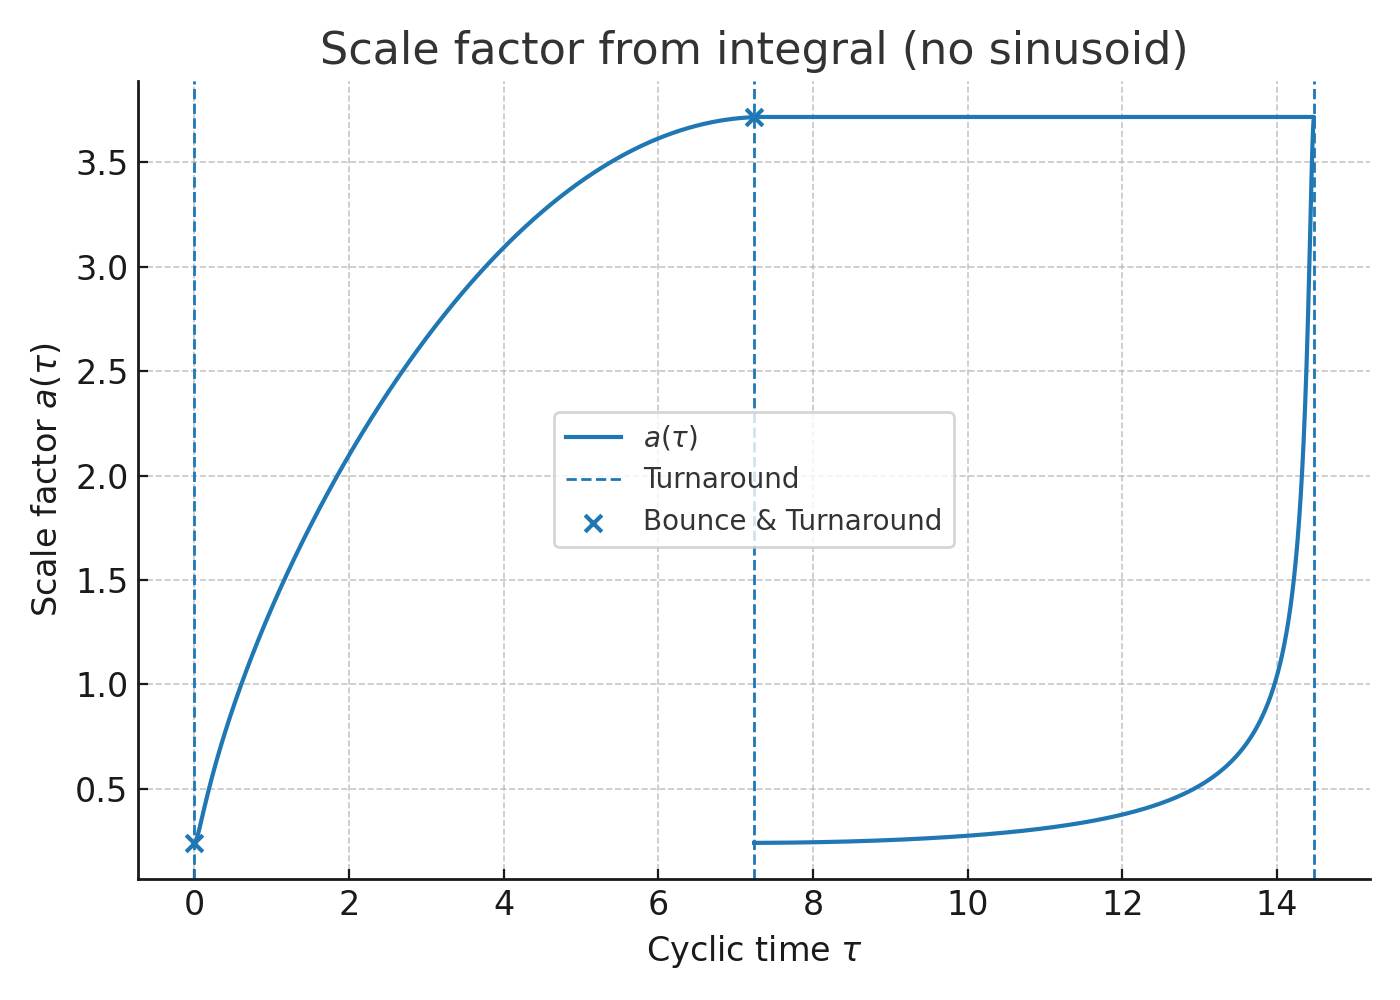
\includegraphics[width=0.78\linewidth]{figures/plot_a_tau_from_integral.png}
\caption{\textbf{Scale factor from the integral solution.}
$a(\tau)$ reconstructed with $\rho_c(R_\tau)$ and $\rho_{\rm CT}(R_\tau)$ included.
Bounce ($a_{\min}$) and turnaround ($a_{\max}$) are marked.}
\end{figure}

\subsection{Effective $H^2(a)$}
\begin{figure}[H]
\centering
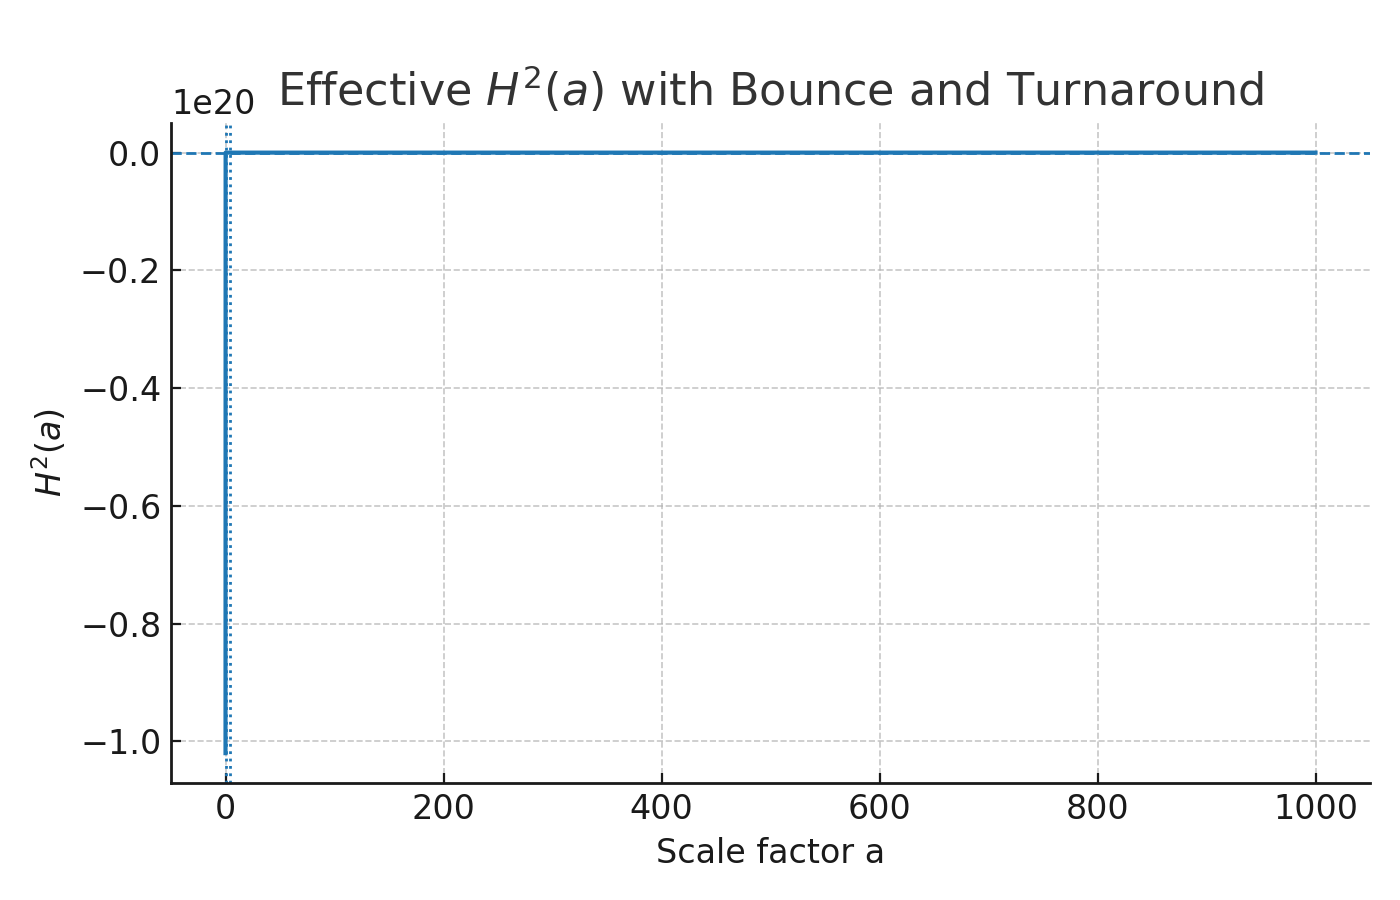
\includegraphics[width=0.78\linewidth]{figures/plot_H2_from_params.png}
\caption{\textbf{Effective $H^2(a)$.}
Numerically computed $H^2(a)$ for the toy parameters, with zeros marking the bounce
and turnaround.}
\end{figure}

\subsection*{Toy Parameters}
\begin{table}[H]
\centering
\small
\setlength{\tabcolsep}{6pt}
\renewcommand{\arraystretch}{1.2}
\begin{tabular}{lcl}
\toprule
Parameter & Value & Description \\
\midrule
$\rho_{m0}$ & $1.0$ & Matter-like density ($\propto a^{-3}$) \\
$\rho_{r0}$ & $0.1$ & Radiation-like density ($\propto a^{-4}$) \\
$\rho_{\rm vac}$ & $-0.02$ & Effective negative term (proxy for $\rho_{\rm CT}$) \\
$\rho_{c}$ & $100.0$ & Critical density (bounce) \\
$k$ & $0$ & Spatial curvature \\
\bottomrule
\end{tabular}
\caption{Toy parameters used to generate the illustrative figures.}
\end{table}

\section{Discussion}
Compared to LQC \cite{Ashtekar2006}, this retains the quantum bounce but introduces a
built-in turnaround. Unlike CCC \cite{Penrose2010}, contraction is preserved.
The model resonates with emergent-time perspectives such as Hartle--Hawking \cite{Hartle1983}
and Rovelli \cite{Rovelli2017}.

\subsection*{Comparison with Other Cyclic Proposals}
\begin{table}[H]
\centering
\footnotesize
\setlength{\tabcolsep}{4pt}
\renewcommand{\arraystretch}{1.25}
\begin{tabularx}{\linewidth}{lYYY}
\toprule
 & \textbf{LQC} & \textbf{CCC (Penrose)} & \textbf{Cyclic 4D-Time (this work)} \\
\midrule
Bounce mechanism
& Quantum-geometry bounce at $\rho=\rho_c$
& None (aeon-to-aeon conformal identification)
& Bounce at $\rho=\rho_c(R_\tau)$ \\
Turnaround mechanism
& None (expansion continues)
& Not applicable
& Negative $\rho_{\rm CT}(R_\tau)$, or equivalently $k>0$ or $\Lambda<0$ \\
Time structure
& Linear, unbounded
& Infinite succession of aeons
& Compact time $\tau\in S^1$ \\
Contraction phase
& Optional/absent
& Removed by conformal rescaling
& Present; closes the cycle \\
Novel element
& Polymer corrections $\rho_c$
& Conformal identification
& Unified bounce+turnaround via closed time \\
\bottomrule
\end{tabularx}
\caption{Comparison of cyclic universe proposals.}
\end{table}

\subsection*{Entropy and the Arrow of Time}
Cyclic models face the entropy problem: why entropy does not accumulate monotonically across
cycles. CCC invokes conformal thinning of massive degrees of freedom. In the closed-time
framework, one may speculate that the compact geometry enforces entropy reset mechanisms
via holographic bounds or quantum information limits. Another possibility, inspired by CCC,
is that massive particles decay away between cycles, thinning entropy carriers before the
next bounce. Alternatively, holographic entropy bounds might cap entropy per cycle,
forcing a reset. These ideas remain speculative, but they provide concrete targets for
future theoretical and observational work. 

\begin{equation}
S \;\leq\; \frac{A}{4G\hbar},
\end{equation}

which represents the Bekenstein--Hawking entropy bound. Future work should test whether
compact time naturally enforces such a cap, preventing monotonic buildup.

\subsection*{Observational Outlook}
\begin{itemize}
    \item \textbf{CMB anomalies:} oscillatory modulation of the primordial power spectrum,
    with scale set by $R_\tau$. For $R_\tau$ of order $10^2$--$10^3$ in Planck units,
    features would appear in the CMB at multipoles $\ell \sim 20$--30. Roughly, features
    scale as $\ell \sim \pi/\theta \sim \pi D_A / R_\tau$, where $D_A$ is the angular
    diameter distance to last scattering. A precise mapping requires perturbation analysis
    in compact time, which is left for future work. Current Planck observations show mild
    low-$\ell$ anomalies that might be consistent with such periodic modulation, although
    their statistical significance remains debated.
    \item \textbf{Gravitational waves:} cyclic bounce signatures in the tensor spectrum,
    potentially observable with next-generation detectors such as LISA or Cosmic Explorer.
    \item \textbf{Entropy cycling:} relic non-Gaussian features or suppressed entropy
    growth as traces of entropy reset between cycles.
\end{itemize}

\paragraph{Bounce as a wavefunction.}
In a Wheeler--DeWitt minisuperspace approximation, $\Psi(a)$ near $a_{\min}$ can be modeled
as Gaussian-peaked. Since $H=0$ at the bounce, extrinsic curvature vanishes and comoving
observers share a common frame.

\section{Conclusions}
We have presented a toy model where compact time controls both bounce and turnaround.
This differs from LQC (bounce only) and CCC (no contraction). While speculative in its
closed-time interpretation, the framework is internally consistent and suggests
falsifiable signatures.

In particular, both the CMB and the primordial gravitational wave background can serve
as observational probes of the compact-time radius $R_\tau$, allowing the model to be
directly constrained by upcoming data.

Perturbations evolve as
\[
v_k''+(k^2-\tfrac{z''}{z})v_k=0,\qquad
\mu_k''+(k^2-\tfrac{a''}{a})\mu_k=0,
\]
where primes denote derivatives with respect to conformal time $\eta$ (distinct from
the periodic cosmic time $\tau$).

\printbibliography

\end{document}
